% siminos/spatiotemp/chapter/trawl.tex
% $Author: mgudorf3 $ $Date: 2020-02-04 11:42:07 -0500 (Tue, 04 Feb 2020) $

%Possible figures
%initial conditions
%final resulting \twots\
%various twots

The numerical methods of \refsect{sect:adjointdescent} and
\refsect{sect:gaussnewton}, and \refsect{sect:gmres}
enable us survey the infinite \spt\ state space by
finding \twots\ which adequately sample the ensemble of
solutions
that solve \refeq{e-kssFb}.
This is possible provided we start with sufficiently good
initial guesses to solve for minimizers of \refeq{e-costfunctional},
where ``good'' initial conditions are any doubly periodic scalar fields
which converge to \twots\ via our numerical optimization.
To demonstrate the efficacy of our \spt\ methods we will
contrast them with conventional methods. Before this, however,
we will first comment on some philosophical differences between
the initial value problem and boundary value problem.
In \refsect{sect:variational} we describe the reformulation
of \refeq{e-ks} without going into much detail of the motivations
to do so. In what follows we hope to convince the reader that
the variational formulation truly is the only chance for studies
of nonlinear chaotic equations.
This body of work is critically dependent
on being able to find exact time invariant solutions of the \KSe.
What do we mean by this precisely?
The nature of the word ``exact'' which is present in many such
discussions (e.g. ``Exact Coherent Structures''\rf{WK04,W01,W02})
is actually rather nebulous..
In fact, the definition was never really meant as a descriptor
of data but rather it was a manner by which to categorize
fundamental solutions of the governing equations\rf{W01}.
We argue that in fact that describing solutions of
the dynamical systems as ``exact'' is disingenuous. In dynamical
systems there is always going to be propagation of error
due to time integration in the presence of a positive Lyapunov
exponent. We will only offer a qualitative description, as
finding bounds on the error in nonlinear dynamical systems
is a tough proposition and can only be done in certain cases\rf{DV01}.
For example, let us take time integration which produces a discrete
representation of a periodic orbit. Even in the best case
scenario where the initial condition yields a
recurrence within machine precision after one period
the trajectory will eventually escape due to magnification
of numerical errors. Other reason why we claim these trajectories
to not be exact is because they can not be reproduced (in a very
strict case, to be fair).
Unless there
is an actual exchange of data there is a zero percent likelyhood
that a time invariant solution will be reproduced exactly by
another computation. Why? Even in the best case scenario wherein the
numerical parameters are identical between the two computations,
the only manner in which the solutions would be exactly the same
is if the same exact initial condition within machine
precision was used with the exact same
numerical methods (we disregard the fact that
same computer would be required as well).
It is straightforward to use the same numerical procedure but
there is no manner by which to procure the same initial condition.
One might argue that this is too strict and the only demand
is that one be ``close enough''. The issue with this
is that this error distorts any further calculations that
may be desired. Once again
one can say that this is not an issue as long as the results are
``close enough'' within some metric but there may come a time
where these error bars compound to produce results that in fact
are not close enough. One such calculation is the linear stability
analysis of solutions. Small errors can have a profound effect
as the calculations are susceptible to numerical overflow and
numerical underflow (numbers getting too large or small, respectively).
We argue that just as one wants to find
quantities which are \textit{topologically invariant} (independent
of coordinate system) we also would
like it to be \textit{numerically invariant}
(independent of numerical method). As we have attempted
to describe, we believe this is a hopeless endeavor
for the initial value problem
but in the context of our \spt\ differential algebraic equations
this is very possible up to the smallest of differences
(machine precision). One might think that the same arguments
apply, but because there is no longer any dynamics we do not
run into the same issues. The reason for this discrepancy is
due to the differing forms of the equations. The differential
algebraic equations (with constraints) uniquely determine solutions
while the dynamical system methods implicitly depend on
the integration scheme being supplied. Therefore if two
computations were performed with the same constraints and
parameters, the solutions would match as much as physically
possible.
In summary of this point, is that there
is already a lack of reproduction of numerical results
in the computational sciences; when you include that the
results are not exactly reproducible the science itself gets
fuzzier over time.

To better convince the reader, we supply some practical
arguments for why the initial value problem is unlikely to
succeed going forward. Perhaps ironically, one of the hardest
components of finding {\po}s in chaotic systems is finding
good candidates for initial conditions.
Historically, initial conditions
are produced by finding the local minima of the \emph{recurrence
function}\rf{pchaot,duguet08,ChaKer12,STGS18}
\beq
R(t,\period{}) = \frac{|u(t+\period{})-u(t)|}{|u(t)|}
\,.
\ee{recurrfunct}

One starts by generating a long-time trajectory $u(t)$ embedded in the
strange attractor, \ie, with the initial transient thrown away. Next one
computes the pairwise distance
between the present $u(t)$ and future $u(t+\period{})$ points
on the trajectory for each $t$ and $0<\period{}<t$. Whenever the value of the
recurrence function falls beneath some preset tolerance value, $u(t)$ is
presumed to lie near a {\po} of period $\approx \period{}$, and fed into a
Newton routine or other numerical method
as an initial guess. Frequently, especially for short \po s,
Newton routine returns a nearby \po\ for which, by definition
$R(t,\period{})=0$.
The problems with time-series recurrence methods are described
in what follows.
Trajectories of ``nearby'' points diverge exponentially, so
in high dimensions the likelihood of a ``near'' recurrence can be very
small.
More importantly, the norm by which ``nearby'' recurrence
\refeq{recurrfunct} is measured is largely arbitrary; typically, one uses
$L_2$ (Euclidean) norm. No norm used historically in near-recurrence
searches incorporates the geometry of dynamical foliation of the
\statesp, \ie, what the recurrence function flags as a pair of ``nearby''
points $u(t),u(t+\period{})$ may be two states that lie on different folds of
stable-unstable manifolds, close in the full \statesp\ norm, but following
dramatically different paths (think of a phase space orbit that has
returned to a given configuration space point, but moving with
different momenta).
Cases such as these represent false
positives, because they will not converge to a solution
upon application of numerical methods. The only
numerical way (as opposed to somehow including geometrical information
of the strange attractor)
to account for this is to
decrease the numerical tolerance of
recurrences, but this has its own host of problems.
Specifically, it can have a dramatic effect on the
number of false negatives where local
minima of \refeq{recurrfunct} are missed due to the
numerical integration ``stepping over''
the minima unintentionally.
This can be fixed by shortening the step
size of the integration scheme, $\Delta t$
at the expense of computational time.
Another approach for reducing the number
of false negatives would be to go the opposite
direction and relax the tolerance
for determining recurrences.
This unfortunately does not
work either because while it decreases the number of false
negatives it increases the number of false
positives.
Yet another alternative is to instantiate a more complex
numerical routine to account for these false negatives
such as an adaptive time step integrator; when a
lax tolerance of \refeq{recurrfunct} is achieved,
diminish the step size to see if the strict
tolerance is achieved. In practice
it seems more fruitful to ignore these misses and
just hope to find the \po\ with a later segment of
the integrated trajectory. This strategy seems to
lose its merit as the dynamical system becomes ``more chaotic''.
Not only do recurrences become less frequent, but usually
the number of computational variables needs to be
increased to resolve the increasingly complex behavior
of the solutions.

These weaknesses of recurrence methods are well known
and improvements are constantly being made.
For instance, a recent development compares
more than just the difference between state space points.
                    \toCB
Methods that minimize the distance between \emph{segments} of \statesp\
trajectories should be much more robust.
For example, in Page and Kerswell\rf{PagKer19} dynamic mode decomposition
(DMD)\rf{Schmid10,Schmid11} approach, the \spt\ data in form of a time
series of spatial snapshots yields a low-dimensional approximation to the
local tangent space. This, coupled with identification of repeated
harmonics in the DMD eigenvalue spectrum, makes possible detection of \po
s in short time series, as short as a quarter of period of a given \po,
\ie, much before any \statesp\ recurrence.
While Page \& Kerswell replacement of \statesp\ points by \statesp\
trajectories is a much needed improvement over the pairwise point
distances of traditional time-recurrence methods, the method still
presupposes an arbitrarily imposed spatial extent \speriod{}, and searches
for periodicities \period{} in time. Our \spt\ formulation takes the next
step, and seeks for \twots\ for whom both periodicities
$(\speriod{},\period{})$ are intrinsic to the solution itself. That is to say,
they are kept as variables which requires the solving
the corresponding augmented system of equations. The spirit of
their method is almost in line with ours,
they utilize more information to improve their comparisons.
The variational methods on the other hand
utilize more information and also
have the added benefit of the topological constraint of being
doubly periodic by definition.

This long exposition on the recurrence method is
because there are not many techniques available
to the initial value formulation. Analogously
in our \spt\
formulation the techniques all involve
initializing a grid of \spt\ \Fcs, but
the manner in which to do so can vary greatly.
The crux of the decision on method to use
is how to balance quality
versus computational time.
It may be better (and we act like it is)
to accept crude initial conditions
the method minimizes the amount of computational time.
This might seem unfair after the
lambasting of recurrence methods but generally we agree that
our choice is not a good one; but it works and is very simple,
which reinforces how potent the variational formulation can be.
Our general rule is that
the initial condition generation should take much less time
and be much less complex than the actual optimization procedure!
We initiate a spectral grid of \spt\ Fourier modes
with random numbers. Technically the
coefficients are not completely random,
the spectra are modified to better impersonate
the spectra of \twots by accounting for
physical scales.
The general rule, without accounting for
equation specific scales, is that in
periodic directions we require that
$|\ukj |\to 0$ as $k,j \to \infty$ sufficiently fast.
This of course
is computationally trivial and merely
requires element-wise multiplication by
an appropriate scaling template.

This method has drawn skepticism
from others experienced
with chaotic PDEs (especially finding {\po}s),
regarding our initial condition generation procedure.
A randomly assigned spectrum
not going to be an solution to \refeq{e-kssFb},
or even close to a solution for that matter.
The critique usually arises from practitioners
of inexact Newton's methods such as GMRES\rf{Saad1986}.
This technique is only viable if the
accompanying numerical methods are reliable and robust; it took
a non-trivial amount of time in order to get to
the point where we could find \twots\ from essentially random noise.
The fact that these methods work in the face of skepticism
seem to reinforce how useful they are.
A cavaet before we proceed,
this method may very well be applicable only to the \KSe due to its
dissipative nature. We have not tested whether the added benefit
from a \spt\ formulation can generalize to more complex
systems such as those governed by the Navier-Stokes equations.


\begin{figure}
\begin{minipage}[height=.05\textheight]{.5\textwidth}
\centering
\small{\texttt{(a)}} \\
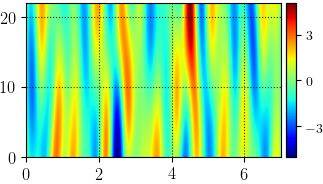
\includegraphics[width=.8\textwidth,height=.2\textheight]{MNG_ppoinitial}
\end{minipage}
\begin{minipage}[height=.2\textheight]{.5\textwidth}
\centering
\small{\texttt{(b)}} \\
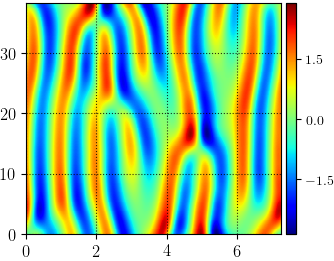
\includegraphics[width=.8\textwidth,height=.3\textheight]{MNG_ppofinal}
\end{minipage}
\begin{minipage}[height=.2\textheight]{.5\textwidth}
\centering
\small{\texttt{(c)}} \\
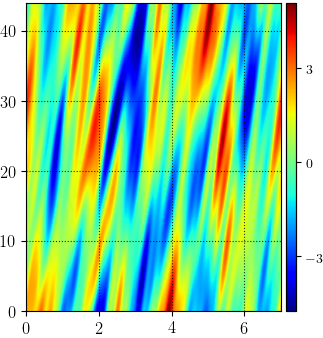
\includegraphics[width=.8\textwidth,height=.39\textheight]{MNG_rpoinitial}
\end{minipage}
\begin{minipage}[height=.2\textheight]{.5\textwidth}
\centering
\small{\texttt{(d)}} \\
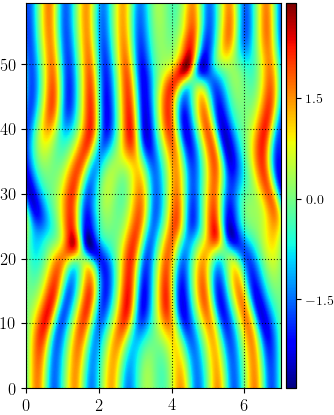
\includegraphics[width=.8\textwidth,height=.48\textheight]{MNG_rpofinal}
\end{minipage}
\caption{ \label{fig:KStrawl}
(a) Initial condition for \twot\ with shift-reflection symmetry, defined on
$\speriod{}=44,\period{}=44$ (fundamental domain). (b) Converged \twot\
resulting from optimization of (a), $\speriod{}= 45.58\dots$,$\period{}= 76.46\dots$.
(c) Initial condition with spatial translation symmetry (shown in co-moving reference frame),
$\speriod{}=44,\period{}=44$. (d) Converged \twot\ resulting from optimization
of (c), $\speriod{} = 44.01\dots$,$\period{}=59.36\dots$,}
\end{figure}

There are alternative methods which we
predict would have greater efficiencies
in terms of convergence.
By taking our library of solutions we can average their
\spt\ Fourier modes to create a template for the ``typical'' spectrum
that different classes of solutions exhibit. There are a number
of things that must be handled carefully, for instance,
for different \spt\ domain sizes the \Fcs\ do not represent
modes with the same frequency so they do not directly map onto
one another. The best way of accounting for the differing domain
sizes is the ``bin'' the frequency data is a method
akin to a histogram. There is another alternative
idea which is hypothetically possible but unclear
whether it is realized.
Our hypothesis is that every \twot\ is comprised of
shadowing of small \spt\ \twots, a topic which we discuss in
much more detail in \refsect{sect:tiles}. If this is
indeed the case then this should be exhibited by
the spectra of the general solution. Therefore,
an additional manner initial conditions could be
created is to take utilize the spectra of just the
tiles.
Looking to the future it has also been put forward that \spt\ methods
will be able to better capitalize on advances in computing, specifically
the increase in number of computational cores\rf{WGBGQ13}.
The idea is that in the future computational speed will not be able
to keep pace with the number of computational cores, and so
one should begin to think in parallel.
Our \spt\ formulation is in the same spirit but unfortunately
we are precluded from the same subdivision that Wang \etal\rf{WGBGQ13} use
because we use periodic boundary conditions. Their idea
is that by subdividing \spt\ domains into subdomains, the equations
being solved locally on each subdomain, in parallel, and then combined
together at their boundaries implicitly. This does not allow for
periodic boundary conditions implying that a \spt\ Fourier basis
is a poor choice. One would want to switch
to either a finite difference scheme or (preferably) a Chebyshev
collocation method in conjunction with new boundary conditions.
On the other side of this discussion, the main
disadvantage of the \spt\ formulation is the increased
number of variables.
To represent the discretization of
a point in the dynamical system's state space we
might use $M$ spatial Fourier modes. The \spt\ equivalent would
be a $N \times M$ \spt\ discretization. In addition, the convergence of
the temporal modes is typically slower than spatial modes because
the time derivatives are of first order. Therefore, not
only must we increase the number of variables by a factor of $N$
but also $N$ will typically be larger than $M$, implying a practical
lower bound of $M^2$ for the number of computational variables. This
quadratic scaling is of course dramatically worse than the $\mathcal{O}(M)$
scaling. The effect of this increase in dimensionality precludes
us from using direct methods such as Newton's method,
as the number of entries of any linearization matrix scales approximately
like $M^4$.

%%%
%under construction
%%%
We are now able to produce initial conditions and use them
to find converged \twots. Now that we will
describe some of the numerical details of our implementation
to better illustrate the typical manner with which we find solutions.
In order to adequately sample
the space of solutions of the \KSe, the
initial conditions were formed
on various \spt\ domain sizes and symmetry types. Specifically
the vast majority of initial conditions generated had parameters
that fit within the ranges $L \in [22,66]$,$T \in [20,180]$.
The computational demands increase as the \spt\ domain size increases
and so if we do not have a good reason to search for large solutions we
probably shouldn't. Our hypothesis is that larger solutions
are comprised of shadowing events of small \spt\ \twots.
As such, we hope that by sampling the space of solutions
up to a manageable size we can capture the fundamental (small)
\spt\ patterns need to describe any \twot.
Once the \spt\ domain size has been chosen the next step
is to decide on the size of the discretization. Typically we choose
integers which are powers of two for the spatial and temporal
discretization sizes because fast Fourier transforms
exploit this. For our
numerical experiments we have found
$N=\text{max}[2^{\text{int}(\log \lfloor T \rfloor+1)},64]$,
$M=\text{max}[2^{\text{int}(\log \lfloor L \rfloor)},32]$ to
work well for these \spt\ domain sizes.
The numerical methods we employ and these parameter values
have a sufficient rate of convergence to be useful. We measure
this efficiency by merely running trials at a distribution
of parameter values as demonstrated in
%reffig{fig:convergencerate} when produced
In our experience, the most important detail seems to be
the size of the \spt\ discretization; there seems to be
a computational sweet spot of discretization sizes where all
important scales are resolved but there are not an excess of
\Fcs.
The general symptoms
of over-resolving and under-resolving are as follows.
For over-resolving the main effect is
a substantial drop off in convergence rate. Consider
the following: in terms of \spt\ \Fcs, over resolving
a solution manifests as including \spt\ \Fcs\ whose
amplitude is near zero. This makes our numerical problem
more ill conditioned and therefore makes it harder to
solve using direct methods; qualitatively this
deterioration is a result of linearly dependent columns
in the Newton system.
For under-resolving there are two typical behaviors; one
is that solutions will converge to \eqva\ and \reqva more often.
%Are qualitative descriptions bad?
Another
result of low resolution is that converged solutions are
produced which look different from the typical
\KSe\ solutions. What we mean by this is that the solutions
will look ``bumpy'' due to the absence of higher frequency modes.

%N,M efficiency at different T,L ->
%T,L efficiency with most efficient N,M


%\begin{figure}
%\begin{minipage}[height=.05\textheight]{.5\textwidth}
%\centering
%\small{\texttt{(a)}} \\
%\includegraphics[width=.8\textwidth,height=.2\textheight]{MNG_underresolvedtwot}
%\end{minipage}
%\begin{minipage}[height=.2\textheight]{.5\textwidth}
%\centering
%\small{\texttt{(b)}} \\
%\includegraphics[width=.8\textwidth,height=.3\textheight]{MNG_resolvedtwot}
%\end{minipage}
%\begin{minipage}[height=.2\textheight]{.5\textwidth}
%\caption{ \label{fig:underresolve}
%(a) A \twot\ of the \KSe\ defined on the \spt\ domain $L=$,$T=$
%which has been under-resolved numerically. (b) The result of reconverging
%(a) with a larger \spt\ discretization size, $L=$,$T=$. The discrepancy
%between the \spt\ domain sizes of (a) and (b) is a result of the
%parameters $L,T$ being solved for in the optimization process.}
%\end{figure}

Examples of the types of initial conditions and the resulting converged \twots\
are displayed in \PCedit{\reffig{fig:KStrawl}}. No special concessions
are made between the varying initial conditions other than those associated
with continuous and discrete symmetries.
%Include the convergence rate information for various initial condition methods?
%only really use one.

In summary, our \spt\ formulation involves no time integrations and is
thus free of their exponential instabilities. It allows us to
find a large number of numerically accurate \twots\
with comparatively small computational cost.
This allows
us to test our main hypothesis which describes larger \spt\ \twots\
in terms of fundamental ``tiles'' which we shall see in \refsect{sect:tiles}
and \refsect{sect:glue}. Namely, we will demonstrate that it is possible to
take combine subdomains of known solutions to find even more solutions.
These methods exemplify the general idea of a self-sustaining process
in Navier-Stokes flows, in which the general process of sustained
turbulence is described via the interactions of a few fundamental
patterns realized in fluid flows\rf{W97}. By construction their
self-sustaining processes are time dependent; for us however, we
merely are combining patterns and see which are admissible.
Their model is an attempt to describe complex behavior with a
relatively simple model.
%This may be a stretch
This type of modeling can loosely
be interpreted as a dimensional reduction because it attempts
to describe temporal patterns with a small number of ``variables''.
Our \spt\ combinations however do not suffer any reduction in complexity
as we use exact \spt\ solutions of \refeq{e-ks} to describe
all possible patterns.
